\documentclass[../../Rapport RayTracer]{subfiles}

\begin{document}


Afin de parser n'importe quel fichier au format pov, la méthode qui a été retenu est celle du pattern State. Ce pattern s'est révélé être le plus adapté pour implémenter un automate à états finis. Voici, ci-dessous, le diagramme de classe de notre pattern state avec les classes d'état qui l'implémentent:

\begin{figure}[h!]
	\adjustbox{center}{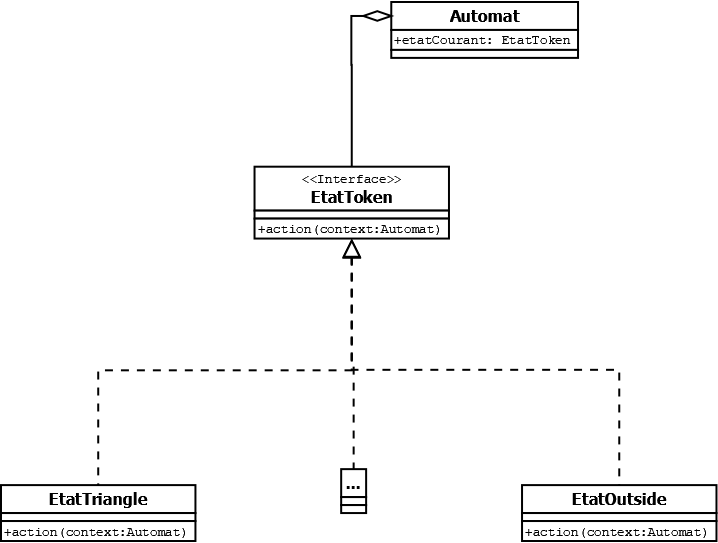
\includegraphics[width=1\textwidth]{diagrammes/pattern_state.png}}
	
	\caption{Diagramme du pattern state appliqué à notre parser}
	\label{diagrammePatternState}
\end{figure}
\FloatBarrier

Ce pattern est composé d'une interface EtatToken qui définit une méthode action qui servira à parser le bon objet. Ensuite, on implémente ce que l'on appelle des classes d'état qui redéfinissent la méthode action et font tout le traitement de la figure. Ces classes correspondent à un seul objet/figure à la fois à l'exception de la classe EtatSpherePlane dont on parlera plus tard. Cette interface est donc en quelque sorte le modèle d'un état.
C'est ensuite la Classe Automat qui s'occupe d'appeler les différents états. Voici un exemple d'appel d'état lorsque l'on tombe sur un objet camera:



\end{document}